\section{Results}
\label{sec:results}

\subsection{Experiment 1: Forgetting Pressure Accelerates Generalization}

\Tabref{tab:exp1} presents the main results. Increasing weight decay from 0 to 1.0 reduces the average grokking step from 17,850 to 583---a \textbf{30.6$\times$ speedup}. The relationship is monotonic: every increase in weight decay produces a corresponding decrease in grokking time.

\begin{table}[t]
    \centering
    \caption{Effect of weight decay (forgetting pressure) on grokking dynamics. Higher weight decay monotonically accelerates generalization while increasing per-example forgetting events. Best grokking speed in \textbf{bold}.}
    \begin{tabular}{@{}lcccc@{}}
        \toprule
        Weight Decay & Avg Grok Step & Std & Avg FE/Example & Test Acc \\
        \midrule
        0.0   & 17,850 & 6,224 & 0.11 & 0.996 \\
        0.001 & 17,183 & 6,465 & 0.11 & 0.997 \\
        0.01  & 11,917 & 5,255 & 0.11 & 0.998 \\
        0.1   & 2,850  & 632   & 0.11 & 1.000 \\
        1.0   & \textbf{583} & \textbf{29} & 1.20 & 1.000 \\
        \bottomrule
    \end{tabular}
    \label{tab:exp1}
\end{table}

The Spearman rank correlation between weight decay and grokking step is $\rho = -0.88$ ($p < 0.00002$), confirming a strong monotonic relationship. The effect size between $\lambda = 0$ and $\lambda = 0.1$ is Cohen's $d = 3.91$---an extremely large effect by conventional standards.

\begin{figure}[t]
    \centering
    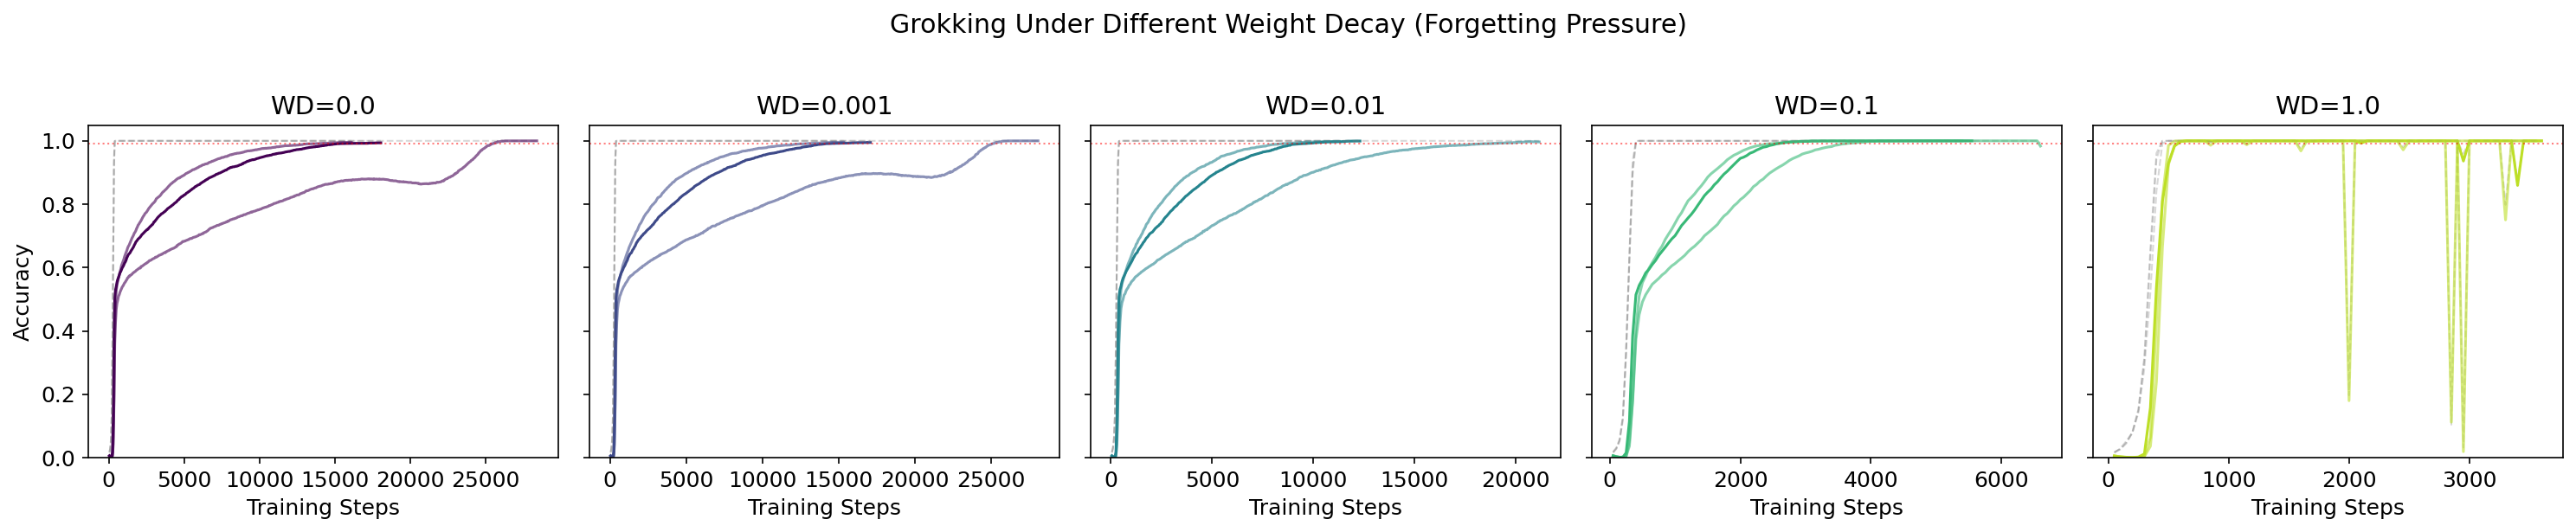
\includegraphics[width=0.95\linewidth]{figures/exp1_grokking_curves.png}
    \caption{Test accuracy curves across weight decay levels. Higher weight decay (darker curves) leads to dramatically faster grokking. At $\lambda = 0$, the model memorizes for ${\sim}$17,000 steps before generalizing; at $\lambda = 1.0$, generalization occurs within 600 steps.}
    \label{fig:grokking_curves}
\end{figure}

\para{Forgetting events track generalization.} At $\lambda = 0$, examples average only 0.11 forgetting events, and ${\sim}$90\% of examples are unforgettable (learned once, never forgotten). At $\lambda = 1.0$, forgetting events increase to 1.20 per example, and only ${\sim}$1\% of examples are unforgettable (\figref{fig:grok_steps}). The model that forgets more per-example learns the general rule faster.

\begin{figure}[t]
    \centering
    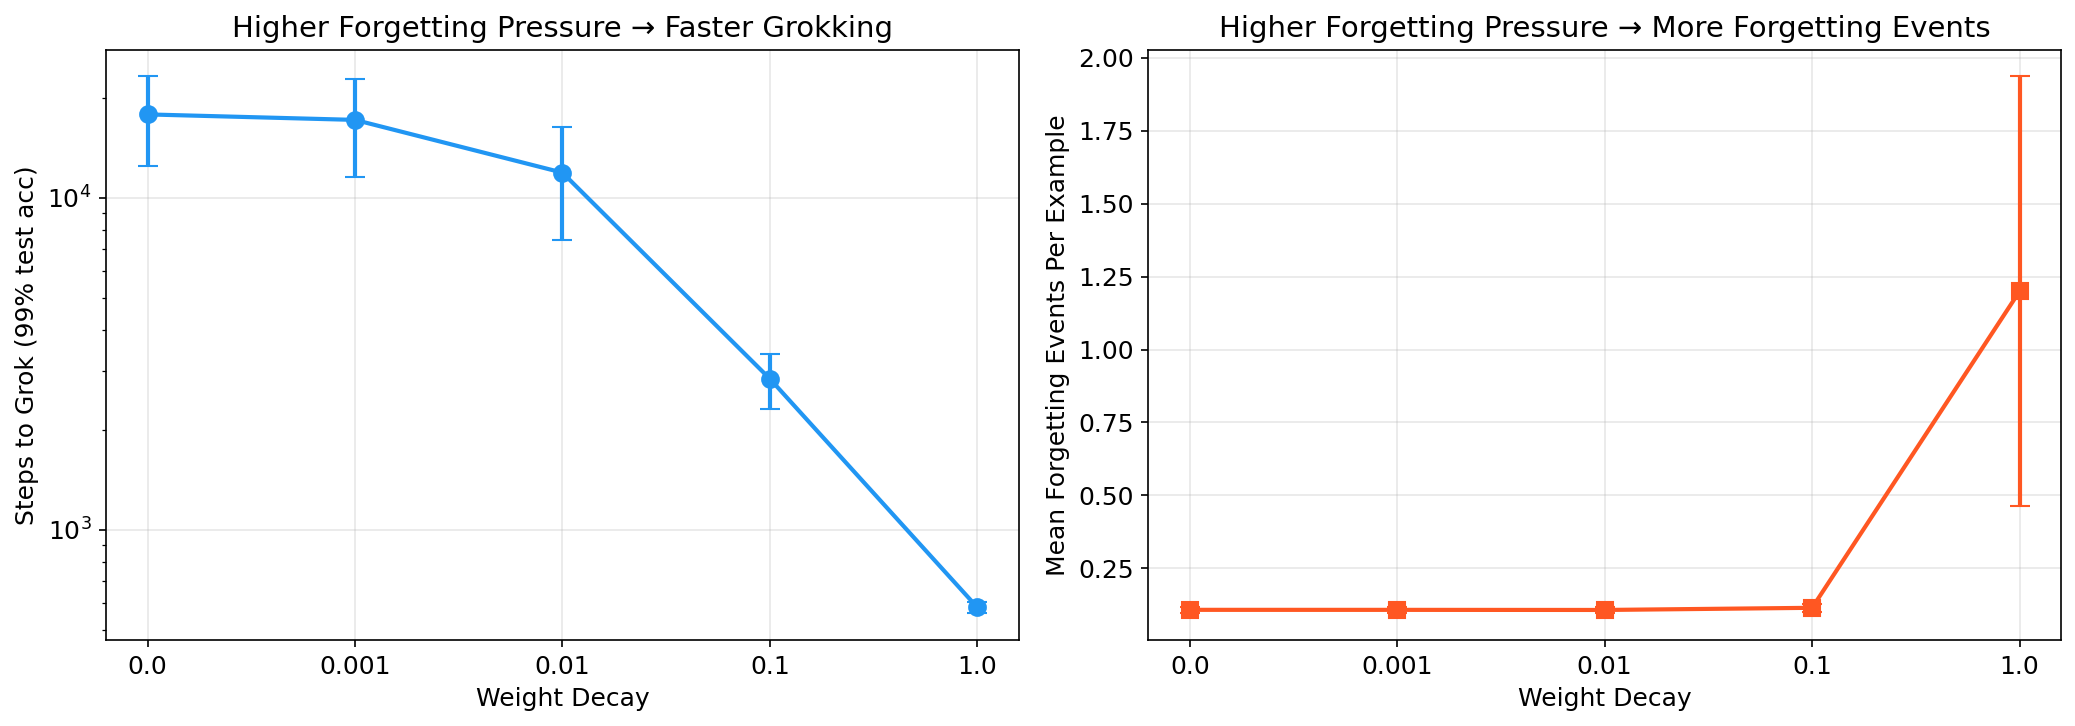
\includegraphics[width=0.95\linewidth]{figures/exp1_grok_steps_and_forgetting.png}
    \caption{Grokking steps (left axis) and forgetting events per example (right axis) as a function of weight decay. The sharp increase in forgetting events at $\lambda = 1.0$ coincides with a 30$\times$ reduction in grokking time, directly linking per-example forgetting to generalization speed.}
    \label{fig:grok_steps}
\end{figure}

\para{Oscillatory dynamics at high weight decay.} At $\lambda = 1.0$, we observe periodic ``collapses'' where training accuracy drops to near-random before rapidly recovering. This oscillatory behavior is consistent with the memorization-compression cycles described by \citet{yu2025memorization}: the model repeatedly memorizes, is pushed away from the memorized solution by weight decay, and eventually settles on a generalizable representation that is robust to the forgetting pressure.

\subsection{Experiment 2: Duplication Slows Generalization}

\Tabref{tab:exp2} shows that increasing data duplication slows grokking. Moving from 1$\times$ to 8$\times$ duplication increases the average grokking step from 583 to 800---a 37\% slowdown. All conditions eventually grok to 100\% test accuracy, but redundant examples provide diminishing returns.

\begin{table}[t]
    \centering
    \caption{Effect of data duplication on grokking dynamics (all with $\lambda = 1.0$). Higher duplication slows generalization. FE = forgetting events per example for duplicated vs.\ non-duplicated subsets.}
    \begin{tabular}{@{}lcccc@{}}
        \toprule
        Duplication & Avg Grok Step & Dup FE & Non-Dup FE & Test Acc \\
        \midrule
        1$\times$ & \textbf{583} & 1.19 & 1.20 & 1.000 \\
        2$\times$ & 600 & 0.24 & 0.20 & 1.000 \\
        4$\times$ & 683 & 2.73 & 2.75 & 1.000 \\
        8$\times$ & 800 & 1.67 & 1.95 & 1.000 \\
        \bottomrule
    \end{tabular}
    \label{tab:exp2}
\end{table}

\begin{figure}[t]
    \centering
    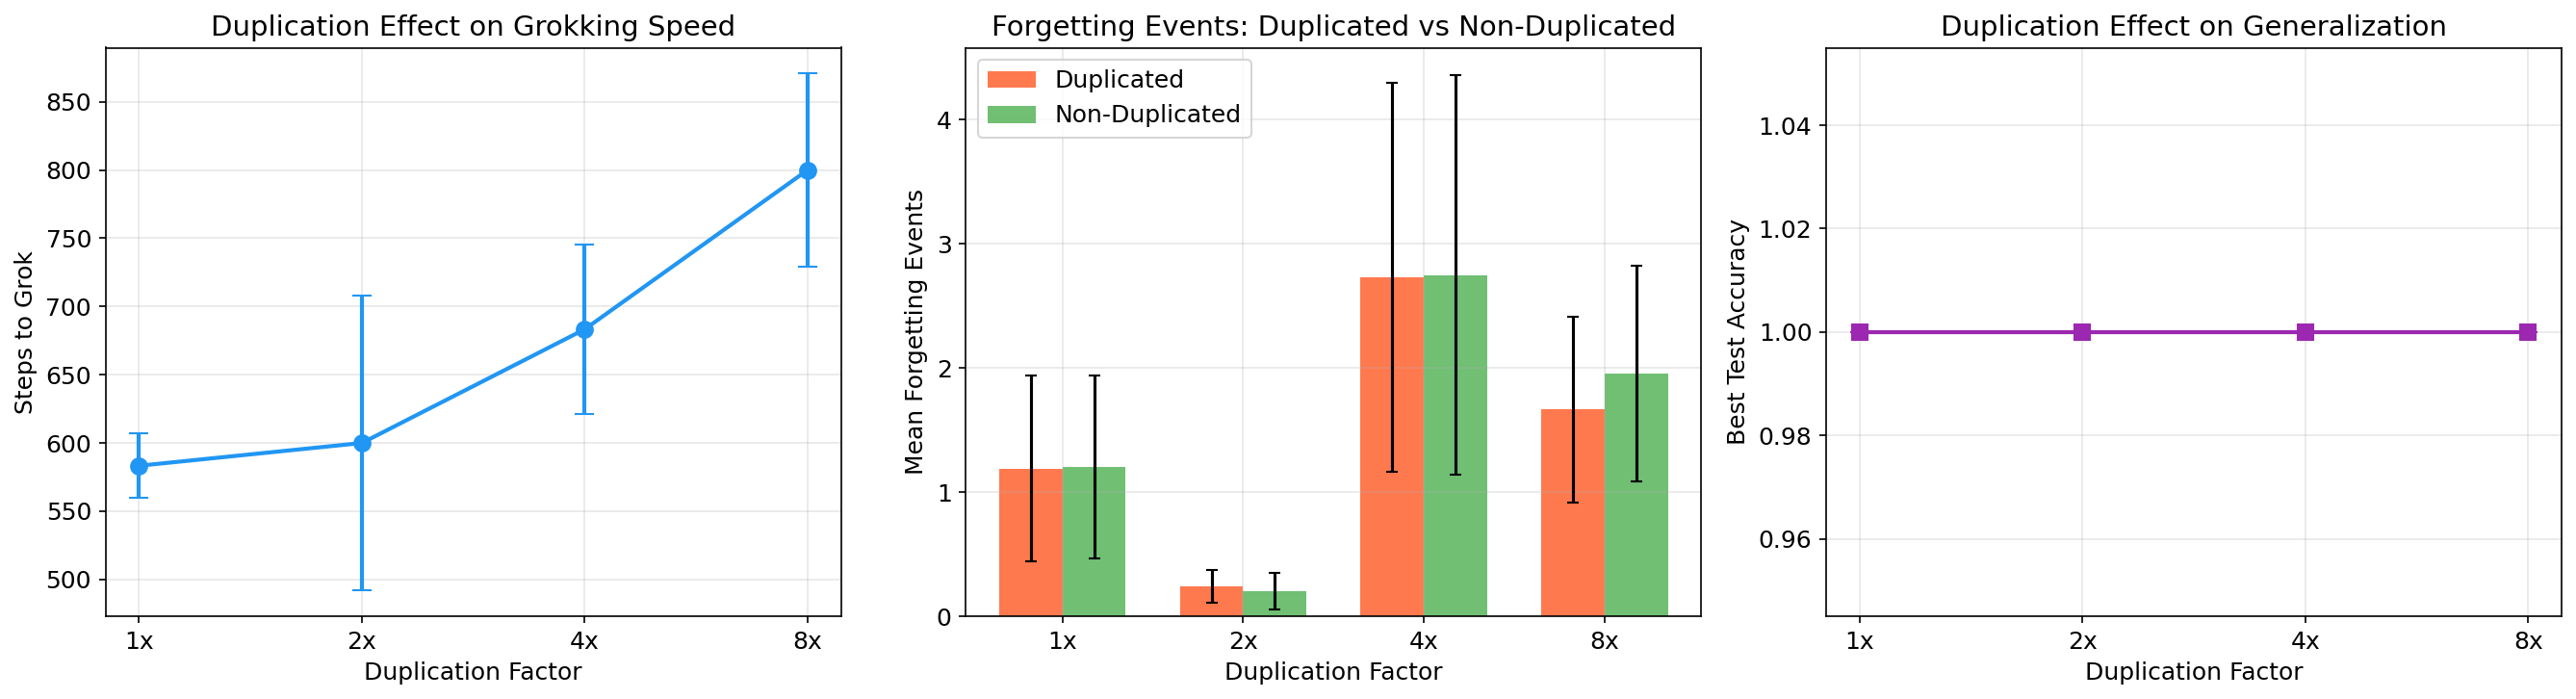
\includegraphics[width=0.95\linewidth]{figures/exp2_duplication_analysis.png}
    \caption{Effect of data duplication on grokking speed and forgetting events. \figleft Grokking step increases with duplication level. \figright Forgetting events for duplicated vs.\ non-duplicated examples show no consistent advantage for duplicated examples.}
    \label{fig:duplication}
\end{figure}

The difference in forgetting events between duplicated and non-duplicated examples is not consistently large. At $\lambda = 1.0$, the strong forgetting pressure largely compensates for duplication effects. We expect the duplication penalty to be larger at lower weight decay levels, where the model has less implicit forgetting to counteract redundancy.

\subsection{Experiment 3: Optimal Forgetting Exists}

\Tabref{tab:exp3} compares forgetting interventions. All conditions achieve 100\% grokking rate, but grokking speed and data efficiency vary substantially.

\begin{table}[t]
    \centering
    \caption{Comparison of forgetting interventions. Grok rate is the fraction of seeds achieving $\geq$99\% test accuracy. Data efficiency is area under the test accuracy curve (higher is better). Best results per column in \textbf{bold}.}
    \begin{tabular}{@{}lccc@{}}
        \toprule
        Intervention & Grok Rate & Avg Grok Step & Data Efficiency \\
        \midrule
        Baseline ($\lambda = 1.0$) & 100\% & 583 & 0.881 \\
        Dropout 0.1  & 100\% & 800 & 0.840 \\
        Dropout 0.3  & 100\% & 7,433 & 0.597 \\
        Noise (small) & 100\% & 583 & 0.878 \\
        Noise (large) & 100\% & 583 & 0.700 \\
        Reset (gentle) & 100\% & \textbf{550} & 0.851 \\
        Reset (aggressive) & 100\% & 567 & 0.788 \\
        \bottomrule
    \end{tabular}
    \label{tab:exp3}
\end{table}

\begin{figure}[t]
    \centering
    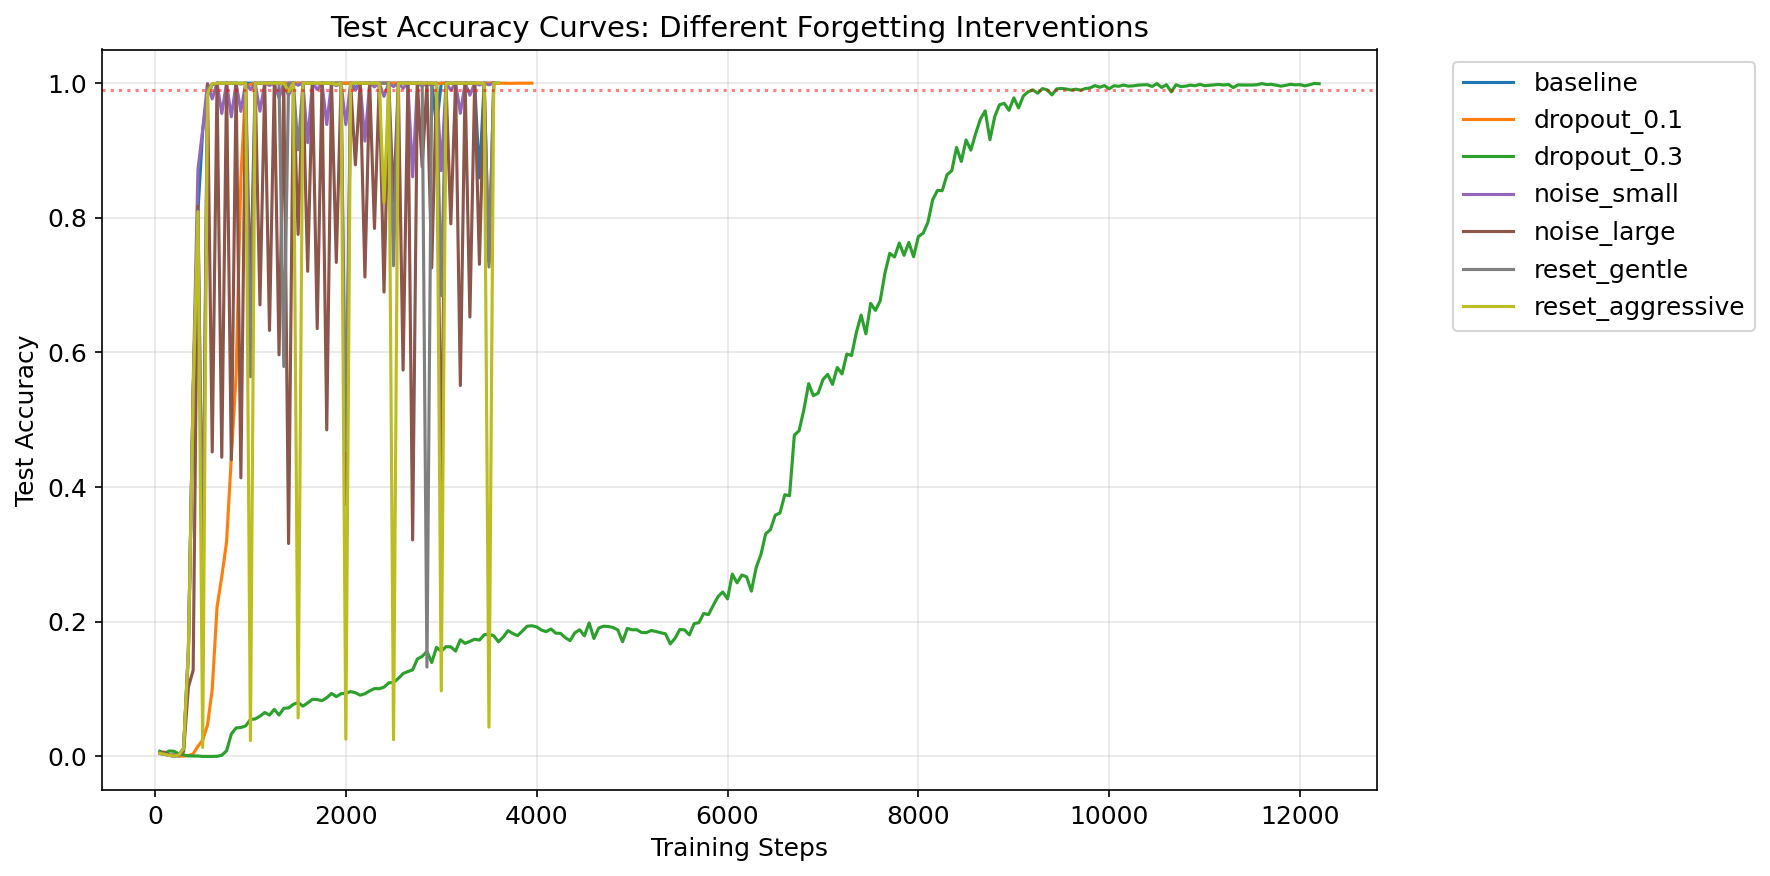
\includegraphics[width=0.95\linewidth]{figures/exp3_learning_curves.png}
    \caption{Learning curves for all forgetting interventions. Gentle interventions (reset gentle, noise small) perform comparably to the weight decay baseline, while excessive forgetting (dropout 0.3) catastrophically delays generalization.}
    \label{fig:interventions}
\end{figure}

\para{Weight decay is a strong forgetting mechanism.} The baseline with $\lambda = 1.0$ achieves the best data efficiency (0.881) and competitive grokking speed (583 steps). Weight decay specifically penalizes large, example-specific weights---exactly the kind of weights that encode memorized solutions---while preserving smaller, structured weights that encode generalizable rules.

\para{Excessive forgetting is catastrophic.} Dropout at rate 0.3 delays grokking by 12.7$\times$ relative to baseline (7,433 vs.\ 583 steps) and achieves the worst data efficiency (0.597). Unlike weight decay, which targets memorized parameters, dropout is indiscriminate---it disrupts both memorized and generalizable representations equally.

\para{Gentle interventions match or improve on baseline.} Reset (gentle) achieves the fastest grokking (550 steps), marginally outperforming baseline. Small noise injection matches baseline grokking speed with comparable data efficiency. These results suggest that the relationship between forgetting and generalization follows an inverted-U shape: moderate forgetting accelerates generalization, but excessive forgetting prevents it.

\subsection{Summary Figure}

\Figref{fig:summary} presents a combined view of all three experiments, showing the consistent relationship between forgetting pressure and generalization across conditions.

\begin{figure}[t]
    \centering
    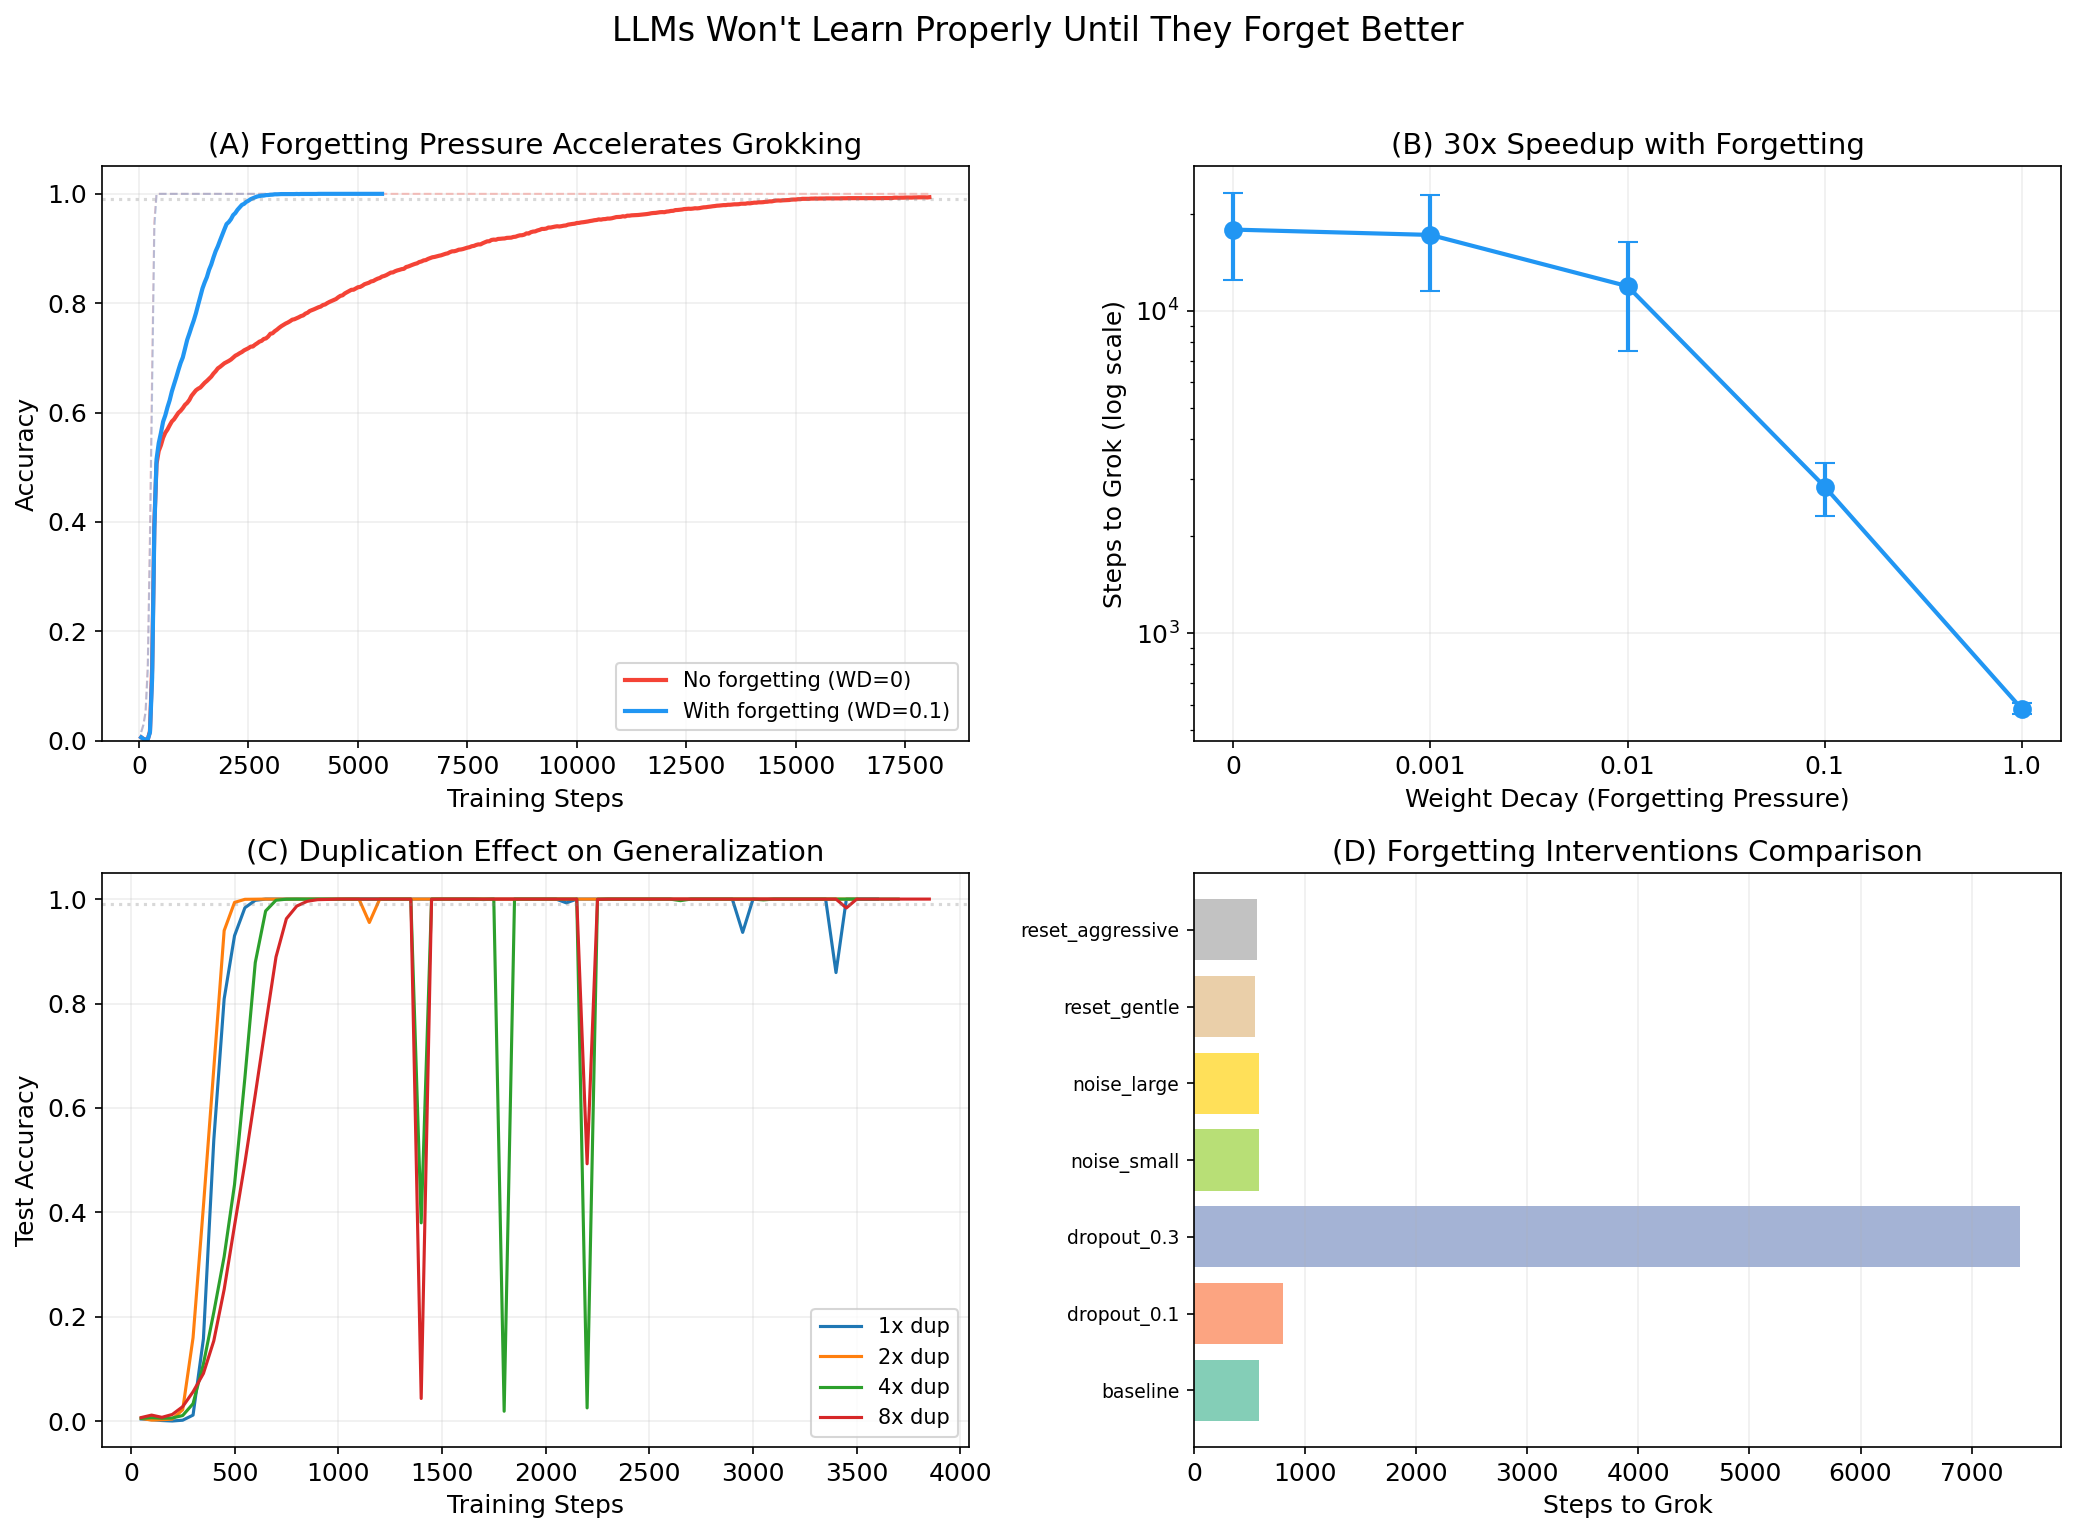
\includegraphics[width=0.95\linewidth]{figures/summary_figure.png}
    \caption{Summary of all three experiments. \captiona Weight decay monotonically accelerates grokking (30$\times$ speedup). \captionb Per-example forgetting events increase sharply at high weight decay. \captionc Data duplication slows generalization by up to 37\%. \captiond Forgetting interventions reveal an optimal forgetting level---too little or too much hurts.}
    \label{fig:summary}
\end{figure}
